\documentclass[11pt,twocolumn]{article} 

\usepackage[spanish]{babel}
\usepackage{url, hyperref}
\usepackage{tabularx}
\usepackage{graphicx}
\DeclareGraphicsExtensions{.png}
\title{
\vspace{-3cm}   
Sistemas de Autentificaci\'on\\
basados en RFID
}

\author{ 
Jorge Rubens Lipa Challapa\\
\\
Universidad Mayor de San Sim\'on \\
Sociedad Cient\'ifica de Estudiantes de Sistemas e Inform\'atica\\
\url {http://www.scesi.org/}
}

\date{ \today }

\begin{document}
\maketitle

\begin{abstract} 
Los sistemas de autentificaci\'on ofrecen un control de 
acceso para un grupo determinado de personas y ofrecer datos estad\'isticos 
referentes a las entradas y salidas del personal donde se procesara para 
proveer informaci\'on muy valiosa al momento de realizar seguimiento, 
frecuencia de accesos y controlando los permisos de acceso al ambiente.\\
\\
 Pudiendo ser utilizado en diferentes \'ambitos y \'areas de
 trabajo donde se requiera una autentificaci\'on digital que permita el \\
 ingreso de un grupo de personas.
\end{abstract}

\section{Introducci\'on}
Uno de los problemas de seguridad mas frecuentes,  a sido el control de acceso 
a ambientes que requieren de una identificaci\'on. Esto se debe a  la 
cantidad de usuarios, tama\~no del ambiente o el tipo de acceso.\\ 
Las diferentes soluciones existentes llegan a tener alg\'un tipo de dificultad, 
ya sea por tiempo, costo y tambien sobre el personal encargado donde la 
implementaci\'on llega a ser laboriosa y compleja para los encargados.\\
\\
Los sistema de autentificacion basados en RFID, permitir\'an, el manejo y 
control de personal y seguimiento de actividades a todo usuario que necesite 
una verificaci\'on de identidad para ingresar a un ambiente o verificar la 
identidad del usuario.\\
\\
Para esto se utlizara tecnolog\'ias como \textit{ Android, arduino y 
servicios web} esto permitir\'a que un encargado de seguridad o un grupo de 
seguridad gestione el control de acceso del personal de una manera r\'apida 
\textit{(Open Hardware)} y simple a un costo reducido \textit{(Open Source)} .\\

\section{Antecedentes}

Generalmente se ve muy a menudo que todos los ambientes  con un nivel de acceso 
tengan una seguridad de acuerdo a un est\'andar y regido por un protocolo, para 
dar cierta privacidad y confidencialidad, esto puede variar ya que los dispositivos 
de acceso varian en los m\'etodos de autenficaci\'on , validaci\'on y seguimiento 
de las actividades sobre el grupo de personas autentificadas. Esto deja al 
descubierto agujeros de seguridad en el ambiente, que mas tarde se interpretara 
como debilidades y falencias en la seguridad.\\
\\
Para asegurar la confidencialidad y privacidad, de ambientes que requieran un 
control de acceso limitando a un grupo de personas, se llega a la conclusi\'on: 
Estos individuos  requieren de permisos especiales, en este caso roles de 
acceso, para ingresar o realizar actividades que est\'en limitadas por uno o mas  
dispositivo de control. \\

\section{RFID}

RFID, Radio Frequency Identification permite transmitir la identidad de un 
objeto a una frecuencia con que se comunica con un dispositivo que reconoce al 
objeto. Este comportamiento esta basado en el modelo emisor receptor. \\

\begin{figure}[t]
  \begin{center}
    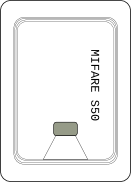
\includegraphics[width=2in]{mifare.png}
  \end{center}

  \caption{\small Dise\~no interno de Mifare S50. Tarjeta de identidad}
  \label{fig-label}
\end{figure}

\section{Tarjeta de identidad}

La tarjeta plástica PVC laminada tamaño ISO estándar: 85,7 x 54 x 0,82 mm, 6gr. aproximadamente, puden llegar a trabajar en frecuencias de : 125KHz, 13,56 MHz, 980Mhz. donde su implementaci\'on varia de acuerdo a la necesidad. cada uno de 
estos objetos de identidad viene integrado con un chip de lectura y escritura, la velocidad de transferencia para la lectura y escritura esta establecida a unos 106 Kbits/s. Esta tarjetas ya viene integradas con una arquitectura de acceso que 
permite ser adecuada de acuerdo a la necesidad. cada uno posee un n\'umero \'unico incluido al momento de la fabricaci\'on.\\
\\
Para las dos primeras frecuencias ya mencionadas el rango de lectura y escritura es de una distancia m\'axima  de 10 cm, los datos pueden permanecer almacenados por al menos 10 a\~nos.\\
\\
Tal como se muestra en la Figura 1. El esquema de la tarjeta de identidad esta dividido en dos partes:\\

\begin{itemize}
	\item Antena de cobre
	\item Microcontrolador
\end{itemize}

La funcionalidad de esta tarjeta varia de acuerdo al uso como ser: para autentificaci\'on, o monetizaci\'on. En la actualidad varios pa\'ises emplean de diferentes formas el uso de los dispositivos de identificicaci\'on, como venta de pasajes para medios de transporte masivo, identificaci\'on en tarjetas de credito, credenciales medicas. inventarios de productos o ganado, inventarios.\\ 

\section{Aporte tecnol\'ogico}

Como una primera liberacion se plaena la implementaci\'on de hardware libres como Arduino impulsara la adopci\'on de los dispositivos electr\'onicos en otras \'areas gracias a la gran variedad de m\'odulos que cuenta y tambi\'en tecnolog\'ias como los servicios web que descentralizaran la informaci\'on y el monitoreo en tiempo real, permitiendo a diferentes dispositivos tener informaci\'on de manera inmediata mediante celulares, tablets, paginas web.\\
\\
Para ello el proyectos Centinela abarcara varios escenarios, desde el control de acceso a eventos sociales, billetera electr\'onico, acceso a parqueos, historial de actividades todos esto utilizando RFID como base para el desarrollo de futuros sistema de identificaci\'on.\\


\section{Proyecto Centinela}

El proyecto Centinela, Control y seguimiento de actividades de acceso para la identificaci\'on personal. Esta basado en tecnolog\'ias  
\textit{ Open source }. Dicho sistema  proveer\'a el acceso a ambientes controlados mediante RFID, los datos ser\'an mandados mediante un servicio web para su procesamiento en un servidor.  Figura \ref{fig-centinela}.\\
\\
Los datos obtenidos se utilizaran para realizar reportes de seguimiento a los usuarios registrados. Los dispositivos de recolecci\'on estan basados en dise\~no construidos con arduino, mientras  que para los dispositivos m\'oviles que tengan NFC se manejaran mediante una aplicaci\'on movil o dispositivo prefabricado que se conectara con el servicio web para el procesamiento de datos.\\

\begin{figure}[!h]
  \begin{center}
    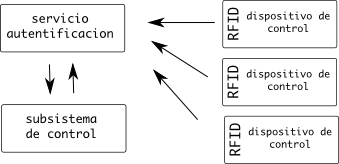
\includegraphics[width=3in]{diagram.png}
  \end{center}

  \caption{\small Modelo de implementaci\'on para el Proyecto Centinela.}
  \label{fig-centinela}
\end{figure}

\subsection{Subsistema -  Evento Social}

Este subsistema esta encargado de controlar el acceso a participantes a un 
evento social, Con ello se permite realizar un registro de la asistencia 
al evento y tener un registro de actividades que se necesiten en el evento.
\\

Para ello el dispositivo de control debe tener registrado previamente al 
individuo en el sistema, posteriormente limitar el acceso a eventos donde 
se haya registrado.\\

Los componentes del sistema se basan en en modelo principal. ya que este 
es un subsistema. este es limitado por el dispositivo de control y registro.
En otros subsistas se vera que los dispositivos de control varian de acuerdo
a su uso.\\

\begin{figure}[!h]
  \begin{center}
    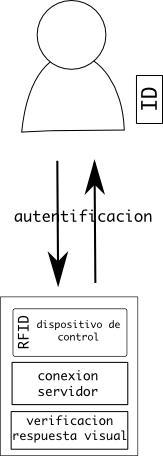
\includegraphics[width=1in]{social-event.png}
  \end{center}

  \caption{\small Proceso de autentificaci\'on.}
  \label{fig-centinela}
\end{figure}



\subsection{Subsistema - Garaje}

El subsistema de garaje, esta pensado para parqueos que necesitan registros 
exaustivos de entradas y salidas de las movilidades para poder saber cuanto 
tiempo a estado barado en el estacionamiento.\\

El principio de autentificaci\'on se similar al subsistema Evento Social.Pero 
difiere en la tarjeta de identificaci\'on, ya que esta debe ser leida desde 
una gran distancia.\\

El problema de la lectura de la distancia es manejada con  el dispositovo de
 control, para ello se utilizara lectores del ultra alta frecuencia. Estos 
 dispositivos claramente no pueden ser creados con las placas arduino, para 
 ello se recurre a productos externos que faciltar esa tarea.\\
 

\begin{figure}[!h]
  \begin{center}
    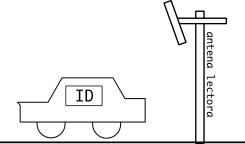
\includegraphics[width=2.5in]{garage.png}
  \end{center}

  \caption{\small Proceso de autentificaci\'on para movilidades.}
  \label{fig-centinela}
\end{figure} 

\subsection{Subsistema - Almacen}

Destinado para el inventariado de objetos que  almacenen en amplios lotes 
donde cada uno deba ser catalogado, clasificado y expedido segun la afinidad
 del gestor.\\
 
La gran utilidad de rfid en inventarios, reduce de manera dramatica el trabajo 
a los operarios, ya que con una lectura de la tarjeta de identificaci\'on, se 
tendra toda la informacion relevante del objeto en cuestion de segundos, eliminando 
la necesidad de consultar libros, leendo codigos visuales.\\


Para la implementacion de este subsistema los dispositivos de control deben ser 
portables para que el operario pueda realizar una verificaci\'on manual. Para 
laverificaci\'on de grande lotes  el dispositivo portable pierde eficacion, este 
sera remplazado por un lector de mayor alcance.\\

Los dos escenarios planteados, requieren que se tome la decisi\'on de elegir el 
tipo de dispositivo de control, ya que al implementar una la otra se descarta 
inmediatamente.\\

El descarte del dispositivo es a causa del dise\~no de la tarjera de identificaci\'on 
. La misma arquitectura de la tarjeta de control cambia y se necesitara de una elecci\'on 
previa para poder operar el subsistema.\\

\begin{figure}[!h]
  \begin{center}
    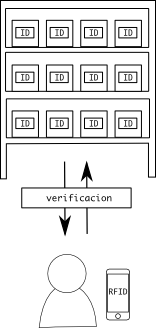
\includegraphics[width=1in]{store.png}
  \end{center}

  \caption{\small Modelo de verificacion individual.}
  \label{fig-centinela}
\end{figure}


\subsection{Subsistema - Billetera}

Orientado a la cargar y recargar de dinero digital \textit{(cr\'edito)} , utilizando la funcionalidad 
"Wallet" (monedero) de las tarjetas Mifare S50. Con esto se podr\'a realizar 
el intercambio de cr\'edito que se asociara a un monto de dinero, pudiendo 
representar una forma de pago o cambio, por ejemplo en un auto bus, pagar 
los pasajes con una identificaci\'on RFID, recargar cr\'editos en un vale 
de descuento y dem\'as usos que tenga que ver con cambios de estado para un 
incremento y decremento.\\

Un dispositivo de control realizara la transacci\'on y guardara los cambios en 
el dispositivo de manera r\'apida. la recargar se har\'a mediante  otro 
dispositivo que guardara los datos de usuarios y la cantidad del incremento 
o decremento.\\

Los Servicios de control se los realizara v\'ia web mediante un servicio web 
compatible con Centinela para verificar la autenticidad de la tarjeta y 
realizar el seguimiento. Figura \ref{fig-pocketpay}.\\



\begin{figure}[!h]
  \begin{center}
    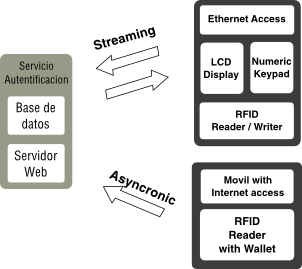
\includegraphics[width=2in]{pocketpay.png}
  \end{center}

  \caption{\small Modelo de implementaci\'on para Billetera.}
  \label{fig-pocketpay}
\end{figure}

\section{Metodolog\'ia de trabajo}  

La para la realizaci\' de los proyectos citados y dar la funcionalidad 
esperada,es necesario  administrar y gestionar la informaci\'on de los usuarios y los 
dispositivos de control donde cada unno varia de acuerdo a la tarea que desempe\~na.

La metodolog\'ia de trabajo se apoyara en la siguientes historias para un posterior 
desarrollo, estas  comprende tres \'areas  que dar\'an como resultado a un 
modelo de trabajo general de todos los subsistemas:\\

	\subsection{ Sistema web }
	
	\begin{description}
		\item [Registro basado en roles] Gesti\'on de los usuarios como el 
		administrador, seguridad y personal com\'un.
		\item [Dispositivos de control] Gesti\'on de los dispositivos de control.
		\item [Seguimiento] Seguimiento de las actividades referentes a las 
		credenciales de autentificaci\'on.
		\item [Reportes de seguimiento] An\'alisis de datos referentes a las 
		actividades de los usuarios autentificados.
	\end{description}
	
	\subsection{Aplicaci\'on para dispositivos portables}		
	
	 \begin{description}
		 \item[Seguimiento de actividad] Seguimiento de procesos de identificaci\'on 
		 a los dispositivos de control.
		 \item[Reporte personal] Reporte de seguimiento de actividad personal.
		 \item[Reporte individual] Informaci\'on relacionada a la tarjeta de identificaci\'on y su objeto.
	 \end{description}
	
	\subsection{Dispositivo electr\'onico}
	
	 \begin{description}
		 \item[Comunicaci\'on con sistema web] Interfaz de acceso al sistema web 
		 mediante una conexi\'on Ethernet.
		 \item[Verificaci\'on de identidad] Recuperaci\'on de informaci\'on de la tarjeta de identificaci\'on.
		 \item[Interacci\'on con usuario] Respuesta a las lecturas realizadas con el dispositivo de control.
	 \end{description}			

\section{Herramientas de Desarrollo}

Se a clasificado las herramientas y dispositivos que servir\'an para la 
culminaci\'on del prototipo inicial, establecidos en las secciones: Dispositivos 
electr\'onicos, Herramientas de prueba, Herramientas de desarrollo.

	\subsection{Dispositivos electr\'onicos }

	Los  dispositivos electr\'onicos que se mencionan est\'an limitados en base 
	al prototipo que se pretende realizar:\\
	
	\begin{enumerate}
		\item Arduino Uno
		\item Raspberry Pi Modelo B
		\item Tarjeta RFID Mifare S50
		\item Tarjeta RFID EM41000 
		\item Lector RFID RS232 13.56 Mhz
		\item Lector RFID RS232 125 khz
		\item M\'odulo de red (arduino) w5100
		\item Ruteador inalambrico y cableado
		\item Tableta o telefono celular con chip NFC
	\end{enumerate}
	
	\subsection{Herramientas de desarrollo}
	
	Esta secci\'on detalla el software que se utilizara para el desarrollo en 
	todos los ambientes de trabajo del proyecto Centinela y PocketPay ,detallando su 
	descripci\'on con la versi\'on y su desempe\~no en un ambiente de producci\'on :
	
	\begin{enumerate}
		\item Apache JBoss v2.2
		\item Play Framework v2.3
		\item PostgreSQL v9.3
		\item Android v4.0.4
		\item Apache Cordova v3.5
		\item Arduino IDE v1.0.5
		\item Apache HBase v2.1
	\end{enumerate}

\section{Conclusiones y recomendaciones}

Con la ayuda de Arduino, Apache, Java  las tecnolog\'ias de RFID llegar\'a a competir  frente a 
productos comerciales, si se compara la funcionalidad. Seg\'un la experiencia 
obtenida a lo largo del desarrollo, los  aspectos t\'ecnicos no son un impedimento 
para que surjan proyectos altamente productivos  y eficientes  utilizando Open Source y Open Hardware.
\\	
Con los respectivos subsistemas, se pretende alentar a terceros a 
que mejoren el software o tengan como base el desarrollo de otros sistema de 
autentificaci\'on basados en RFID. Tanton el aspecto t\'ecnico, como humano ,las 
propuestas ya son suficientemente viables para una implementacion directa.\\


Ya sea para probarlo en un ambiente de prueba o producci\'on, la relativa estabilidad estara basada 
en las propuestas que los desarradores de los sistemas de soporte. Ya que estas pueden posteriormente 
pueden ser adaptadas a un entorno muy espec\'ifico.
\\
Muy pronto veremos que la adopci\'on de la tecnolog\'ia de RFID dara mucho que 
hablar en los siguientes a\~nos gracias a su gran utilidad en la identifiaci\'on.
\\


\section{Referencia Bibliogr\'afica}
	
	\begin{itemize}
		\item  Tedjasaputra, Adi (18 de diciembre 2006). «RFID Tag Attachments». RFID 
		Asia. Consultado el 3 de agosto 2007.
		
		\item Dargan, Gaurav; Johnson,Brian; Panchalingam, Mukunthan; Stratis, 
		Chris (2004), The Use of Radio Frequency Identification as a Replacement for 
		Traditional Barcoding
		
		\item "REST APIs must be hypertext driven by Roy Fielding". Roy.gbiv.com. 
		2008-10-20. Retrieved 2013-02-07.
		
		\item Matthieu Schapranow (2013), "Real-time Security Extensions for EPCglobal
		 Networks: Case Study for the Pharmaceutical Industry"
		 
		 \item Nemai Chandra Karmakar (2010)"Handbook of Smart Antennas for RFID 
		 Systems"
		 
	\end{itemize}
	
\end{document}          